\section{Requisitos Não Funcionais}

\subsection{Escalabilidade}

\begin{itemize}
    \item A aplicação suporta 10 000 requisições ao servidor, para tal deverá ser escalável verticalmente.
\end{itemize}

\subsection{Performance}
\begin{itemize}
    \item  O utilizador não deve esperar mais de 3 segundos, em média, para visualizar novo conteúdo após um clique do rato, a parte gráfica não será o foco principal.
    \item Necessita de uma quantidade maior de espaço em disco para processar o grande volume de dados. Para atender a essa necessidade, o armazenamento disponível deve ser de 1TB de espaço em disco.
\end{itemize}


\subsection{Usabilidade}
\begin{itemize}
    \item A plataforma seguirá os padrões de software já conhecidos, tornando-o fácil de utilizar e de aprender:
    \item Facilidade de aprender: O tempo e o esforço exigido para poder usar o sistema é de 2dias de treino.
    \item Facilidade de uso: Velocidade de execução de tarefas pela adição de atalhos, redução de erros com a implementação de perguntas para determinadas operações no sistema.
    \item Serão Adicionadas teclas de atalho dinâmicas das funcionalidades mais utilizadas de acordo com as requisições do utilizador.
    \begin{figure}[!h]
\centering
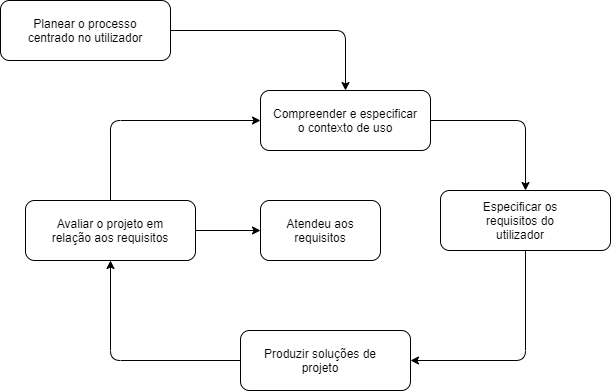
\includegraphics[width=10cm]{Figuras/Usabilidade.png}
\caption{Processo do projeto centrado no utilizador}
\label{d.componentes}
\end{figure}
\end{itemize}
\newpage
\subsection{Disponibilidade}
\begin{itemize}
    \item Pretende-se um sistema disponível em qualquer dispositivo que tenha acesso à internet e um browser instalado, sendo os mais importantes os telemóveis, computadores e tablets.

    \itemr Tendo em conta a necessidade da utilização do portal por parte dos usuários, as atualizações necessárias serão feitas em horas de baixa adesão. O site estará inacessível por um período máximo de duas horas, de forma a não comprometer o seu normal funcionamento.

    \item	Os dados indispensáveis serão alocados também num servidor externo, assim sendo, se o servidor interno estiver inacessível, o utilizador poderá aceder, na mesma, a determinados dados. 
\end{itemize}

\subsection{Manutenção}
\begin{itemize}
    \item	Todos os anos, pelo menos uma vez, o sistema irá sofrer uma intervenção manual, para atualizar a calendarização do ano seguinte;

    \item	Como temos um objetivo inicial simples e concreto, haverá um esforço por parte da equipa de desenvolvedores para adicionar novas funcionalidades e ferramentas que possam vir a ser úteis ao longo do tempo. Esta implementação terá em conta o feedback e as necessidades dos utilizadores;

    \item	A interface do portal será atualizada, conforme a disponibilidade, para evitar que o seu uso frequente se torne monótono e enfadonho, proporcionando assim uma experiência mais agradável para o utilizador.
\end{itemize}
\newpage
\subsection{Segurança}
\begin{itemize}
    \item Sendo uma área de trabalho muito confidencial, o utilizador ao iniciar sessão terá de ter ou um dispositivo móvel ou um email associado à conta para receber um código de segurança (autenticação de dois fatores) de modo a prevenir tentativas de acessos alheios. 
    \item Após a inatividade de um utilizador por mais de 60 minutos a sessão será encerrada automaticamente obrigando-o a efetuar o início de sessão quando retomar.
    \item Sendo uma aplicação WEB este não vai dar autorização ao navegador que guarde os dados (Username e Palavra-Passe) por exemplo numa conta google. Assim no caso de roubo ou perda de algum dispositivo este não terá acesso à aplicação. 
    \item A aplicação deverá cumprir com as políticas de privacidade de dados.
\end{itemize}

\subsection{Cultura}
\begin{itemize}
    \item Tendo em conta que a maioria dos países têm processos distintos na área judicial e o projeto se adequando aos processos portugueses implica a impossibilidade de “vender” o produto para fora de Portugal. Ou seja, para cada país iria necessitar de esquematizações diferentes para podermos “vender” o produto.
\end{itemize}

\subsection{Portabilidade e compatibilidade}
\begin{itemize}
    \item O produto como é uma aplicação WEB poderá ser acedido por qualquer dispositivo em qualquer lugar sem necessitar dos dispositivos pessoais, e sem qualquer tipo de instalação.
    \item Inicialmente a aplicação WEB vai ser suportado para computador e depois também para telemóvel. Sendo uma aplicação WEB não teremos uma carga extra de adaptar tanto para ANDROID como para IOS. Ou seja, a aplicação irá ser compatível com qualquer plataforma.
\end{itemize}

